\documentclass{article}
\usepackage[utf8]{inputenc}
\usepackage[spanish, es-tabla]{babel}
\usepackage{amsmath,amsfonts,amssymb,amsthm,float,bbm}
\usepackage{graphicx}

\author{Jorge Carlos Urteaga \and Víctor R. Martinez}
\title{Falta titulo}
\date{\today}
\decimalpoint

\usepackage{Sweave}
\begin{document}
\Sconcordance{concordance:Final.tex:Final.Rnw:%
1 11 1 1 0 4 1 1 23 12 1 1 4 6 0 1 2 2 1 1 3 2 0 1 2 4 0 1 2 1 1 1 3 6 %
0 1 2 3 1 1 12 70 0 1 1 6 0 1 2 4 1 1 13 12 0 1 1 1 4 3 0 1 4 7 0 1 2 4 %
1 1 3 2 0 1 2 1 0 1 1 1 5 8 0 1 2 2 1 1 6 5 0 3 1 1 2 1 0 1 1 3 0 1 2 2 %
1 1 12 11 0 1 1 1 4 3 0 1 2 5 0 1 2 9 1}


\maketitle




\section{Introducción}
???

\section{Datos}
???

\section{Desarrollo}
\subsection{Procesamiento inicial}
En primer lugar los datos fueron escalados y centrados a media $0$ y varianza $1$ para eliminar el ruido producto de utilizar diferentes unidades entre las variables. Además, si no hacíamos este paso, el procedimiento de reducción de dimensión fallaba por razones aún desconocidas.

\begin{Schunk}
\begin{Sinput}
> #Escalamos las variables a mu = 0, sigma = 1
> alacranes.scaled <- data.frame(scale(alacranes[,-141]),
+                                tipo = alacranes$tipo)
\end{Sinput}
\end{Schunk}

A continuación, reducimos la dimensionalidad del problema utilizando un Análisis de Componentes Principales. Encontramos que con sólo 34 factores eramos capaces de capturar el 95.814\% de la varianza de los datos.

\begin{Schunk}
\begin{Sinput}
> pca <- princomp(~., data=alacranes.scaled[, -141],
+                 cor = TRUE, na.action=na.exclude)
> datos.red <- data.frame(pca$scores[,1:34],
+                         tipo = alacranes.scaled$tipo)
\end{Sinput}
\end{Schunk}

A partir de los componentes más importantes, podemos representar nuestro problema en dos dimensiones para una mejor interpretación de los datos y una primera aproximación al procedimiento que tendremos que utilizar. Como podemos ver en la siguiente figura, los alacranes no venenosos se encuentran agrupados en el centro de los datos rodeados por alacranes venenosos. Es claro que un modelo lineal sería incapaz de separar de manera adecuada los datos, necesitamos un modelo capaz de generar áreas de clasificación circulares.
\begin{Schunk}
\begin{Sinput}
> ggplot(aes(x = Comp.1, y = Comp.2, color = tipo),
+        data = datos.red) + geom_point()
\end{Sinput}
\end{Schunk}
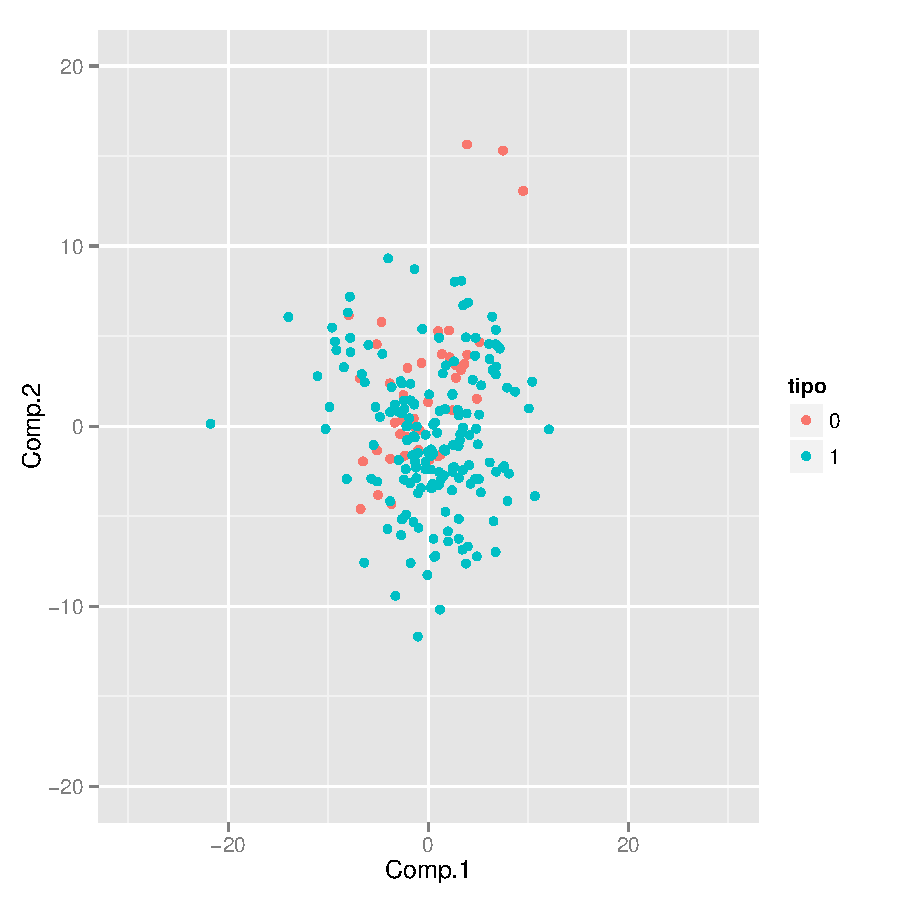
\includegraphics{Final-004}

\subsection{Métodos}
\subsubsection{Red neuronal}
Nuestra primera aproximación al problema fue mediante el uso de una red neuronal. Se entrenó una red neuronal con 12 neuronas en la capa escondida (número determinado de manera empírica) con decaemiento ($10^{-9}$) en un máximo de 1000 iteraciones. Para medir el comportamiento de la red, se utilizó un procedimiento de validación cruzada a 5 iteraciones.
\begin{Schunk}
\begin{Sinput}
> ################################################################
> #                           ANN                                #
> ################################################################
> ann.cross.validation <- sapply(seq(1,5), function(i){
+   train <- datos.red[unlist(kfolds[c(-i)]),]
+   test <- datos.red[kfolds[[i]],]
+   ann <- nnet(tipo ~ ., data = train, size = 12,
+               decay = 1E-9, maxit = 1000)
+   preds <- predict(ann, newdata = test)
+   mean(preds == test$tipo)
+ })
\end{Sinput}
\begin{Soutput}
# weights:  433
initial  value 111.767578 
iter  10 value 31.301331
iter  20 value 0.602869
iter  30 value 0.005277
iter  40 value 0.000424
iter  50 value 0.000133
final  value 0.000090 
converged
# weights:  433
initial  value 124.045574 
iter  10 value 26.695216
iter  20 value 5.138521
iter  30 value 1.593144
iter  40 value 1.395827
iter  50 value 1.386911
iter  60 value 1.386354
iter  70 value 1.386341
iter  80 value 1.386337
final  value 1.386336 
converged
# weights:  433
initial  value 113.515765 
iter  10 value 26.614599
iter  20 value 1.586086
iter  30 value 0.044311
iter  40 value 0.003217
iter  50 value 0.000525
final  value 0.000075 
converged
# weights:  433
initial  value 129.536323 
iter  10 value 28.335465
iter  20 value 3.188184
iter  30 value 1.452323
iter  40 value 1.388088
iter  50 value 1.386454
iter  60 value 1.386360
iter  70 value 1.386333
iter  80 value 1.386313
final  value 1.386312 
converged
# weights:  433
initial  value 163.508054 
iter  10 value 27.943575
iter  20 value 9.324468
iter  30 value 1.948451
iter  40 value 1.401019
iter  50 value 1.387440
iter  60 value 1.386785
iter  70 value 1.386413
iter  80 value 1.386384
iter  90 value 1.386321
final  value 1.386320 
converged
\end{Soutput}
\begin{Sinput}
> mean(ann.cross.validation)
\end{Sinput}
\begin{Soutput}
[1] 0.7246454
\end{Soutput}
\end{Schunk}
En todas las iteraciones de validación cruzada la red convergió. El resultado final fue decepcionante, ya que la red sólo fue capaz de predecir $72.465\%$ de los casos. Como se verá en la siguiente sección, la máquina de soporte vectorial alcanzó mejores resultados en comparación.

\subsection{Máquina de soporte vectorial}
El segundo método estudiado fueron las máquinas de soporte vectorial. Debido a la forma estudiada de los datos se optó por utilizar un \emph{kernel} de tipo radial, con gamma igual a $2$ (determinado empíricamente). De nueva cuenta recurrimos a la validación cruzada de 5 iteraciones para determinar el mejor parámetro de castigo $C$. El espacio explorado fueron las potencias de 10 desde $-3$ hasta $5$. La siguiente figura muestra el promedio de la certeza del estimado junto con sus barras de error estándar con parámetro $C$ en escala logarítmica. Podemos ver que para $C$ pequeñas, el desempeño del estimador es estadísticamente más bajo que para $C > 100$. Además, la certeza del estimador es equivalente para $C \in \{100, 1000, 10000\}$.

\begin{Schunk}
\begin{Sinput}
> cross.validation <- sapply(c(0.001, 0.01, 0.1, 1,
+                              10, 100, 1000, 10000),function(C){
+   medias.C <- sapply(seq(1, 5), function(i){
+     train <- datos.red[unlist(kfolds[c(-i)]),]
+     test <- datos.red[kfolds[[i]],]
+     svm.c <- svm(tipo ~ ., data = train, 
+                  kernel = "radial", gamma = 2,
+                  cost = C)
+     preds <- predict(svm.c, newdata = test)
+     mean(preds == test$tipo)
+   })
+ })
> cross.validation <- t(cross.validation)
> cv.summarize <- data.frame(C = c(0.001, 0.01, 0.1, 1,
+                                  10, 100, 1000, 10000), 
+                            mean = rowSums(cross.validation)/5, 
+                            sd = apply(cross.validation, 1, sd))
> ggplot(aes(x = log(C), y = mean),
+        data = cv.summarize) + geom_errorbar(aes(ymin = mean - sd,
+                                                 ymax = mean + sd, 
+                                                 width=.1)) + geom_point()
\end{Sinput}
\end{Schunk}
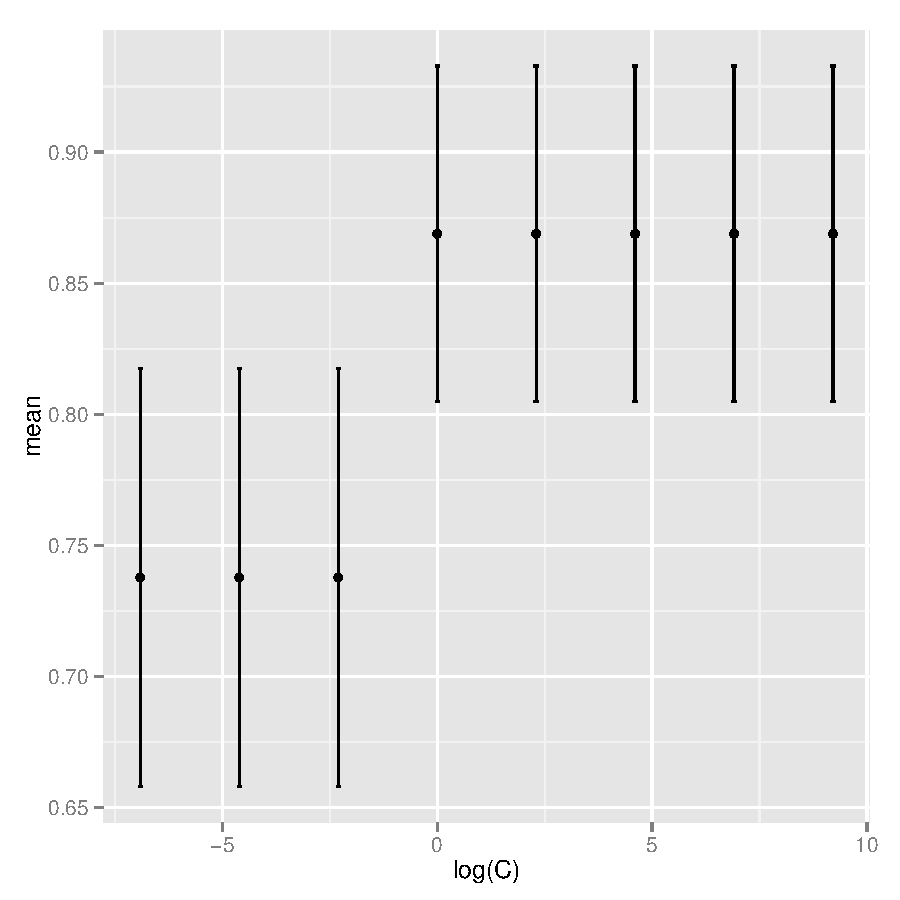
\includegraphics{Final-006}

Para $C > 100$, este clasificador obtuvo una tasa media de clasificación de $85.612\%$ con una desviación estándar de $0.0499$. 

De nueva cuenta, podemos graficar el comportamiento del estimador en dos dimensiones (a partir de los principales factores encontrados). A continuación se muestra como es que el SVM de \emph{kernel} radial con parámetro de castigo $C = 100$ clasifica los puntos del espacio $\mathbb{R}^2$. 

\begin{Schunk}
\begin{Sinput}
> svm.opt <- svm(tipo ~ Comp.1 + Comp.2, data = datos.red,
+                kernel = "radial", gamma = 2, cost = 100)
> dat.x <- expand.grid(Comp.1 = seq(-30,30,0.5),
+                      Comp.2 = seq(-20,20,0.5))
> dat.x$preds.1 <- predict(svm.opt, newdata = dat.x)
> ggplot(dat.x, aes(x = Comp.1, y = Comp.2, 
+                   colour = preds.1)) + 
+   geom_point(size = 1) +
+   geom_point(aes(x = Comp.1, y = Comp.2,
+                  color = tipo), data = datos.red, size = 3)
\end{Sinput}
\end{Schunk}
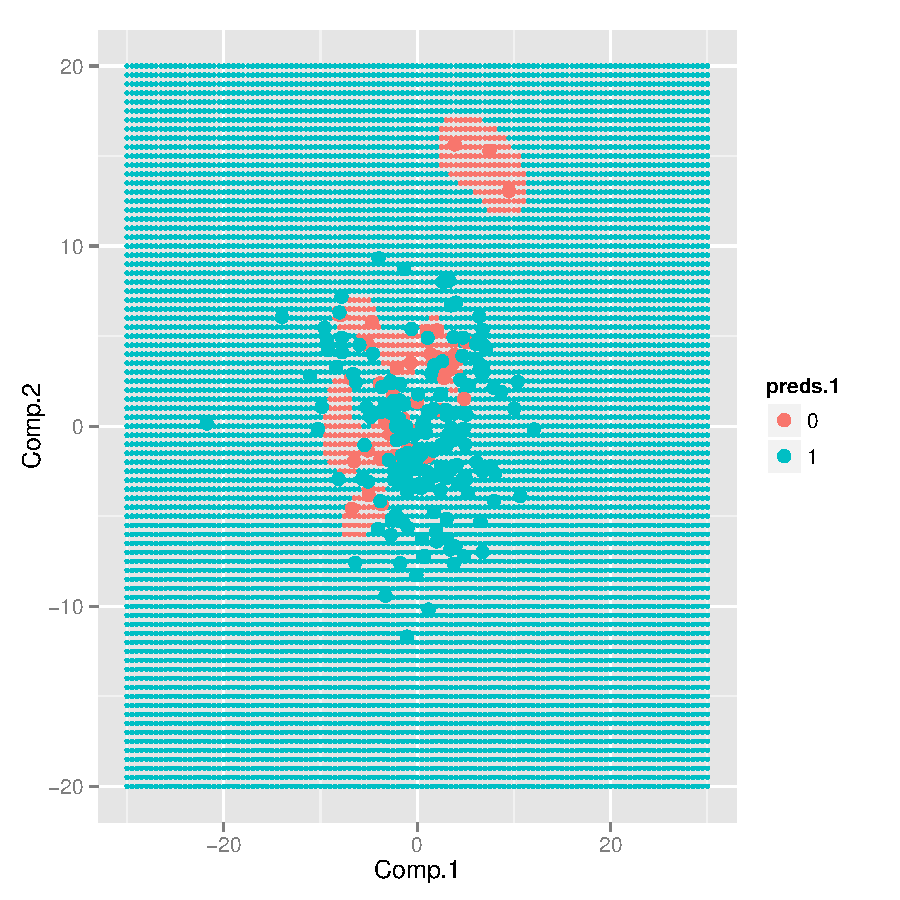
\includegraphics{Final-007}

\subsubsection{Mejorando el modelo: Sesgo y Varianza}
Ahora nos interesa saber si es posible conseguir mejores tasas de clasificación con un clasificador SVM y la manera de hacerlo. Para esto, estudiamos el error de entrenamiento y el error de prueba a distintos tamaños de muestras. Para cada tamaño $n$ era importante asegurarnos que la muestra de entrenamiento tuviera ejemplos de ambas categorías, pues de no ser asi, el modelo SVM no sería capaz de obtener los hiper-planos separadores (pues no hay nada que separar). Por esta razón, utilizamos un muestreo estratificado como se muestra a continuación
\begin{Schunk}
\begin{Sinput}
> # Ocupamos statrified sampling para asegurar que tenemos
> # al menos un elemento de cada clase en la muestra
> # evitando el error de SVM vacio
> ##
> idx.tipo1 <- sample(which(datos.red$tipo == 1), .8 * 174)
> idx.tipo0 <- sample(which(datos.red$tipo == 0), .8 * 62)
> train <- rbind(datos.red[idx.tipo1,], datos.red[idx.tipo0,])
> test <- rbind(datos.red[-idx.tipo0,],datos.red[-idx.tipo1,])
> #Shuffle data
> train <- train[sample(dim(train)[1]),]
> test <- test[sample(dim(test)[1]),]
\end{Sinput}
\end{Schunk}
Al revolver los datos (último paso) nos aseguramos de que, aun en el peor de los casos, una muestra de tamaño 49 tendrá ambas categorías con probabilidad muy alta (cercana a 1). En nuestros experimentos encontramos que el tamaño de la muestra podia ser bastante más bajo. 

Generamos las curvas comparativas de error de entrenamiento y error de prueba para ver si el error que tenemos es producto de sesgo (y no vale la pena agrandar el tamaño de muestra) o varianza (y una muestra más grande podria mejorar nuestro modelo).
\begin{Schunk}
\begin{Sinput}
> errs <- sapply(seq(20, dim(train)[1]), function(i){
+   svm.opt <- svm(tipo ~ ., data = train[1:i,],
+                  kernel = "radial", gamma = 2, cost = 100)
+   #Err train
+   preds.train <- predict(svm.opt, newdata = train[1:i,])
+   err.train <- mean(preds.train != train[1:i,]$tipo)
+   #Err test
+   preds.test <- predict(svm.opt, newdata = test)
+   err.test <- mean(preds.test != test$tipo)
+   list(i, err.train, err.test)
+ })
> errs <- t(errs)
> errs.df.m<- melt(data.frame(i = unlist(errs[,1]),
+                             err.train = unlist(errs[,2]),
+                             err.test = unlist(errs[,3]))
+                  , id=c("i"))
> ggplot(aes(x = i, y = value, colour=variable),
+        data = errs.df.m) + geom_line()
\end{Sinput}
\end{Schunk}
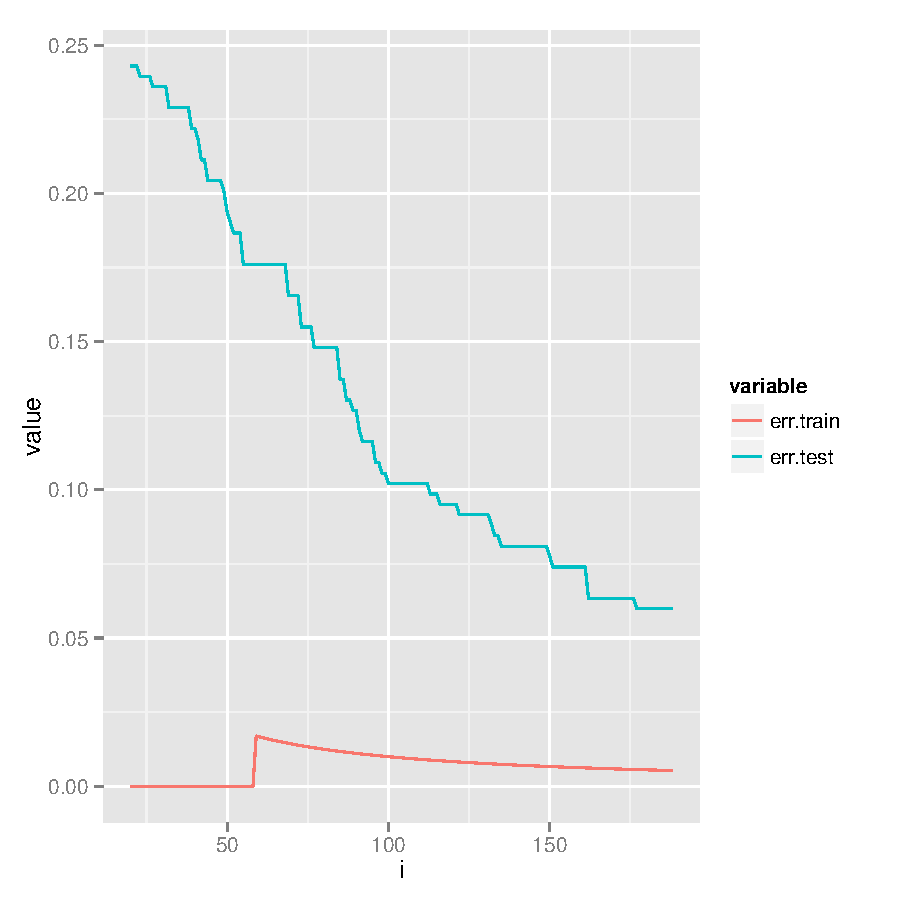
\includegraphics{Final-009}
En esta gráfica podemos observar que las curvas de entrenamiento y validación se encuentran separadas y existe una tendencia de la curva de validación a la baja. Esto sugiere que nuestro error es producto de varianza y que necesitamos obtener una muestra de mayor tamaño para reducir el error.





\section{Resultados}
\section{Conclusiones}

\end{document}
